\chapter{The acoustic space of voice quality in Santiago Laxopa Zapotec} \label{ch:acousticlandscape}

%--------------------------------------------------------------------------
\section{Introduction} \label{sec:acousticlandscape:intro}
%--------------------------------------------------------------------------

This chapter studies the acoustic dimension of voice quality in Santiago Laxopa Zapotec (SLZ) using a Multidimensional Scaling (MDS) analysis of acoustic data. MDS is a statistical method that reduces the dimensionality of a dataset and visualizes the relationships between data points. This study uses MDS to visualize the acoustic space of voice quality in SLZ. This analysis provides information on the acoustic correlates of voice quality in SLZ and contributes to our understanding of the phonetic properties of this underdocumented language.

This study is based on the work conducted by \citet{keatingCrosslanguageAcousticSpace2023} on the acoustic space of voice quality in 11 languages. However, this study focuses on a single language, SLZ, and provides a detailed analysis of the acoustic properties of voice quality in this language. The results of this study will contribute to our understanding of the phonetic properties of SLZ and how the acoustic properties of voice quality in this language compare with other languages.

%--------------------------------------------------------------------------
\section{Methods} \label{sec:acousticlandscape:methods}
%--------------------------------------------------------------------------
%--------------------------------------------------------------------------
\subsection{Participants} \label{sec:acousticlandscape:participants}
%--------------------------------------------------------------------------
This study uses data collected from 10 native speakers of SLZ during the summer of 2022. Participants were recruited from the community of Santiago Laxopa, Oaxaca, Mexico. All participants were native speakers of SLZ. The participants were between 18 and 60 years old and consisted of five males and five females.
%--------------------------------------------------------------------------
\subsection{Recordings} \label{sec:acousticlandscape:recordings} 
%--------------------------------------------------------------------------
The participants were asked to perform a word list elicitation task consisting of 72 words. These words were selected to elicit the entire range of types of voice quality in SLZ, including modal voice, the two kinds of creaky (i.e., checked and rearticulated), and breathy voice. The words were selected based on previous research conducted as part of the Zapotec Language Project at the University of California, Santa Cruz \citep{ZapotecLanguageProject}. 
Because participants were not literate in SLZ, the word list was prompted for them by asking them ``How do you say [word in Spanish]?" by myself and another researcher in Zapotec. Participants were asked to respond with the desired word in the carrier phrase \textit{Shnia' [WORD] chonhe lhas} ``I say [WORD] three times.'' which was repeated three times. These utterances were recorded in a quiet environment using a Zoom H4n digital recorder. The recordings were saved as 16-bit WAV files with a sampling rate of 44.1 kHz.

%--------------------------------------------------------------------------
\subsection{Acoustic measuring} \label{sec:acousticlandscape:analysis}
%--------------------------------------------------------------------------

These resulting audio files were then processed in Praat to isolate the vowel portion of each word. The onset of the vowel was set to the second glottal pulse after the onset, and the offset of the vowel was set to the last glottal pulse before the decrease in amplitude at the end of the vowel \citep{garellekAcousticDiscriminabilityComplex2020}. The vowel was then extracted and saved as a separate file for analysis.

These vowels were fed into VoiceSauce \citep{shueVoiceSauceProgramVoice2011} to generate the acoustic measures for the studies discussed in this dissertation. Because many acoustic measures are based on the fundamental frequency, this measure was calculated using the STRAIGHT algorithm from \citep{kawaharaInstantaneousfrequencybasedPitchExtraction1998} to estimate the fundamental frequency in millisecond (ms) intervals. Once the fundamental frequency is calculated, VoiceSauce then uses an optimization function to locate the harmonics of the spectrum, finding their amplitudes.

VoiceSauce then uses the Snack Sound toolkit \citep{sjolanderSnackSoundToolkit2004} to find the frequencies and bandwidths of the first four formants, also at millisecond intervals. The amplitudes of the harmonics closest to these formant frequencies are located and treated as the amplitudes of the formants. These formant frequencies and bandwidths are used to correct the harmonic amplitudes for the filtering effects of the vocal tract, using \citeauthor{iseliAgeSexVowel2007}'s \citeyear{iseliAgeSexVowel2007} extension of the method employed by \citet{hansonGlottalCharacteristicsFemale1997}. Each vowel was measured across ten equal time intervals, resulting in 22890 data points in total. These measures were then z-scored by speaker to reduce the variation between speakers and provide a way to compare the different measures directly on the similar scales.

%--------------------------------------------------------------------------
\subsection{Data processing} \label{sec:acousticlandscape:processing}
%--------------------------------------------------------------------------
Data points with an absolute z-score value greater than three were considered outliers and excluded from the analyses in the dissertation. The Mahalanobis distance was calculated in the F1-F2 panel within each vowel category. Each data point with a Mahalanobis distance greater than six was considered an outlier and excluded from the analysis.  

Energy was excluded if it had a zero value and then log-transformed to normalize its right-skewed distribution. Afterward, the resulting log-transformed Energy was z-scored, and any data point with a z-score greater than three was excluded. This outlier removal resulted in 1918 data points being removed. 

All data points were then z-scored by speaker to reduce the variation between speakers and provide a way to compare the different measures directly on the same scale.

I then calculated residual H1* for the remaining data points following \citet{chaiH1H2Acoustic2022}. First, a linear mixed effects model was generated with the z-scored H1* as the response variable and the z-scored energy as the fixed effect. The uncorrelated interaction of the z-scored energy by speaker was treated as random. The energy factor resulting from this linear mixed-effects model was extracted. Finally, the z-scored H1* had the product of the z-scored energy and energy factor subtracted from it to produce the residual H1* measure. 

Once these steps were completed, the mean of each combination of phonation and speaker was taken for the fourth through seventh interval of the vowel. This is similar to what \citet{keatingCrosslanguageAcousticSpace2023} did by taking the middle of the vowel for their analysis. This choice minimizes the effect of the onset and offset of the vowel on the acoustic measures, which are more likely to be affected by the surrounding consonants and should give us the most accurate representation of the vowel quality. Because z-scores were used, this resulted in negative measures, which presents a problem for MDS analyses. To correct for this, I added the absolute value of the minimum z-score to each measure. This results in a dataset that still preserves the relative differences in the scores while providing a dataset that is all positive for the MDS analysis.

%--------------------------------------------------------------------------
\subsection{Statistical analysis} \label{sec:acousticlandscape:statistics}
%--------------------------------------------------------------------------

A multidimensional scaling (MDS) analysis is a type of dimensionality reduction in order to visualize the relationships between the data points \citep{kruskalMultidimensionalScaling1978}. Using MDS is especially effective when many variables could contribute to the data. In the case of voice quality, this is especially warranted. 

As shown in \citet{kreimanUnifiedTheoryVoice2014,kreimanValidatingPsychoacousticModel2021,garellekAcousticDiscriminabilityComplex2020}, voice quality is psychoacoustically complex and a single measure is not enough to capture the full range of voice quality. Instead, multiple measures are required that function as cues for the different types of voice quality. For example, a vowel characterized as having a breathy voice has an elevated spectral-slope and a lower harmonics-to-noise ratio than modal voice. A creaky voice has a lowered spectral-slope and a lowered harmonics-to-noise ratio. 

Because MDS analyses that contain many variables can result in rather unmeaningful results, I chose to focus on the speaker by phonation interaction. This allows us to see how speakers differ in their production of the different voice qualities. This choice to focus on speaker by phonation means that each speaker's production of each of the four phonation contrasts is represented as a single point in the MDS plot (e.g., one point for the first speaker's modal voice, one for their checked voice, one for their's rearticulated voice, and one for their breathy voice). This is similar to what \citet{keatingCrosslanguageAcousticSpace2023} did in their study of the acoustic space of voice quality in 11 languages, except that they compared the language by voice quality interaction. Both of these interactions show us similar information. The analysis of speaker by voice quality shows us the acoustic space within a language, while the analysis using language by voice quality shows us the acoustic space between languages.

The MDS analysis was conducted using the \texttt{metaMDS} function in the \texttt{vegan} package \citep{oksanenVeganCommunityEcology2025} in the R programming language \citep{rcoreteamLanguageEnvironmentStatistical2024}. The Manhattan distance was used to estimate the differences between the speaker-by-phonation pairs. Because the distances are non-Euclidean, the MDS analysis was conducted using the non-metric option.

This algorithm resulted in a solution that involves several different dimensions. The number of dimensions retained directly affects how well the original data is captured. Too many dimensions and the data are overfitted; too few, and the data are underfitted. To determine the number of dimensions to retain, I used a scree plot to plot the stress of each dimension. As shown in Figure~\ref{fig:stress_plot}, most of the data is captured in the first four dimensions. These four dimensions were retained for the analysis.

\begin{figure}[!h]
    \centering
    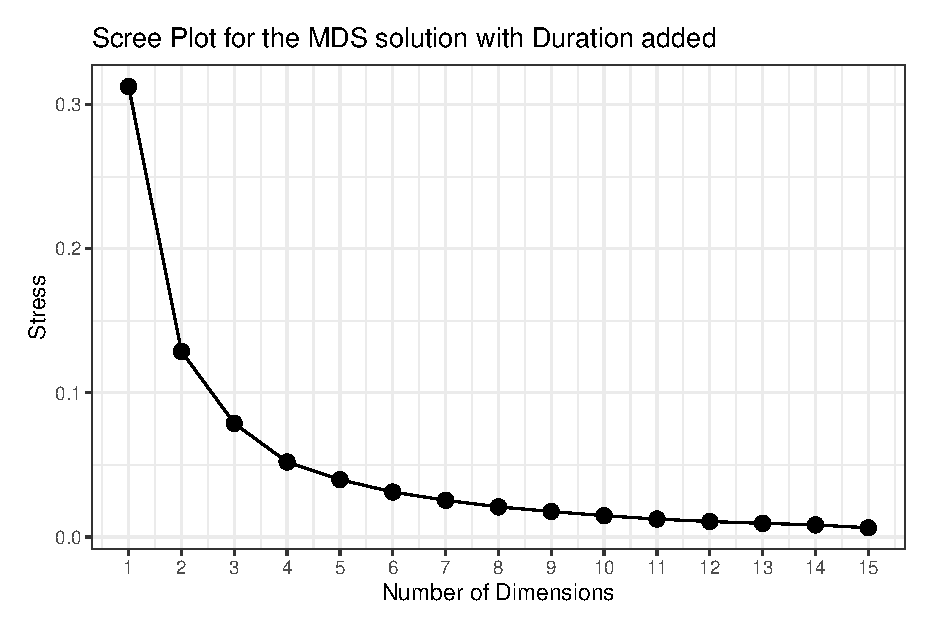
\includegraphics[width = 0.9\linewidth]{images/MDS/stress_plot_dur.eps}
    \caption{Scree plot showing the stress for each dimension for the MDS analysis.}
    \label{fig:stress_plot}
\end{figure}

% \begin{figure}[!h]
%     \centering
%     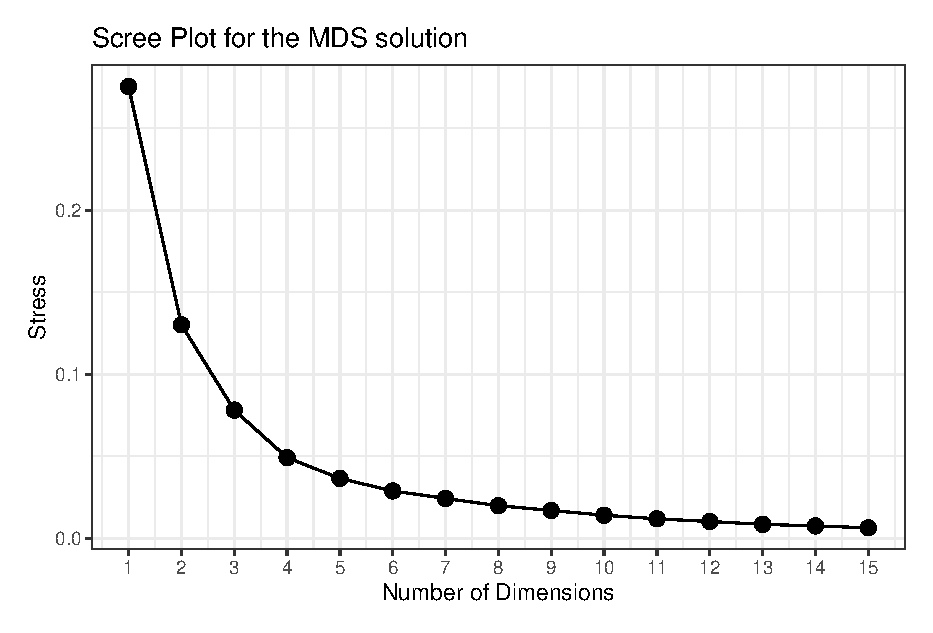
\includegraphics[width = 0.9\linewidth]{images/stress_plot_4:7.eps}
%     \caption{Scree plot showing the stress for each dimension for the MDS analysis.}
%     \label{fig:stress_plot}
% \end{figure}

%--------------------------------------------------------------------------
\section{Results} \label{sec:acousticlandscape:results}
%--------------------------------------------------------------------------
%--------------------------------------------------------------------------
\subsection{Acoustic space of voice quality} \label{sec:acousticlandscape:space}
%--------------------------------------------------------------------------

The results of the MDS analysis show that the acoustical space is represented primarily by a three-dimensional space.\footnote{A 3D plot showing the acoustic space can be found at \href{https://www.mlbrinkerhoff.me/files/3d_plot.html}{https://www.mlbrinkerhoff.me/files/3d_plot.html}.} In all subsequent plots, breathy voice is represented by orange, checked voice with blue, rearticulated voice with green, and modal voice with black. In each of the plots, modal voice is generally more densely packed than the nonmodal voice qualities. This is likely due to the fact that modal voice represents approximately 60\% of the data, while the nonmodal voice qualities represent approximately 40\% of the data. 
% The exact proportions of the data are given in Table~\ref{tab:voice_quality_proportions}.

% \begin{table}[ht]
%     \centering
%     \caption{Proportions of the different voice qualities in the dataset.} 
%     \label{tab:voice_quality_proportions}
%     \begin{tabular}{cccc}
%         \lsptoprule
%         Modal & Breathy & Checked & Rearticulated \\ 
%         \hline
%         0.62707838  &  0.14441805  &  0.09738717  &  0.13111639 \\
%         \lspbottomrule
%     \end{tabular}
% \end{table}

Figure~\ref{fig:nmds12} shows the first dimension plotted against the second dimension. In  this plot, we observe that breathy voice is located in the top left of the plot, modal voice is located in the bottom-center of the plot, and the two types of creaky voices are located to the right of the plot, with checked voice located at the extreme right of the plot, and rearticulated voice located closer to the center. From this plot, we see that the first dimension separates from breathy, modal, and creaky voices. The second dimension separates the modal voice, bottom of the plot, from the nonmodal voice qualities, top of the plot.

\begin{figure}[!ht]
    \centering
    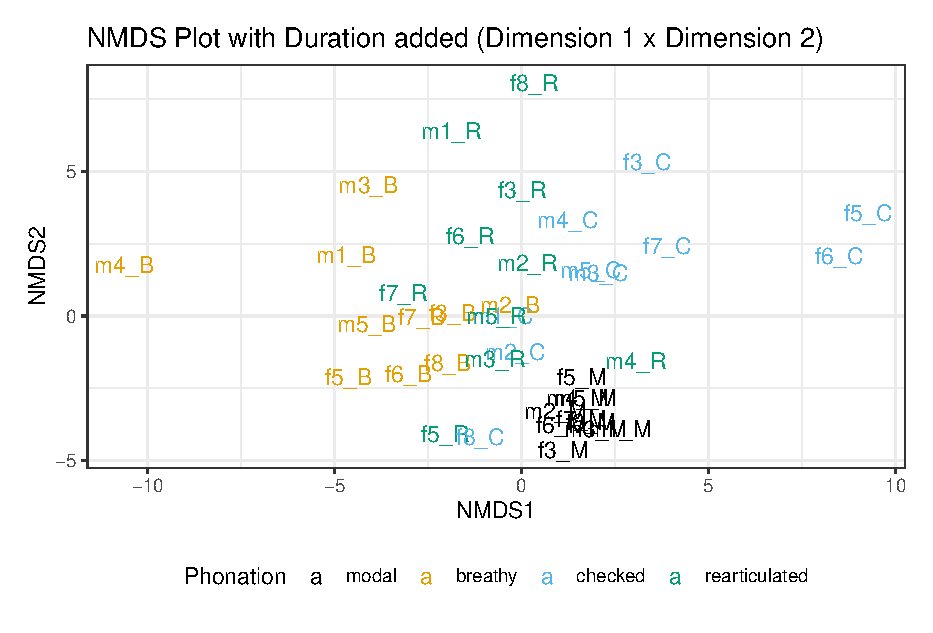
\includegraphics[width = 0.9\linewidth]{images/MDS/nmds12_dur.eps}
    \caption{Two-dimensional MDS solution showing the first and second dimensions.}
    \label{fig:nmds12}
\end{figure}

\begin{figure}[!h]
    \centering
    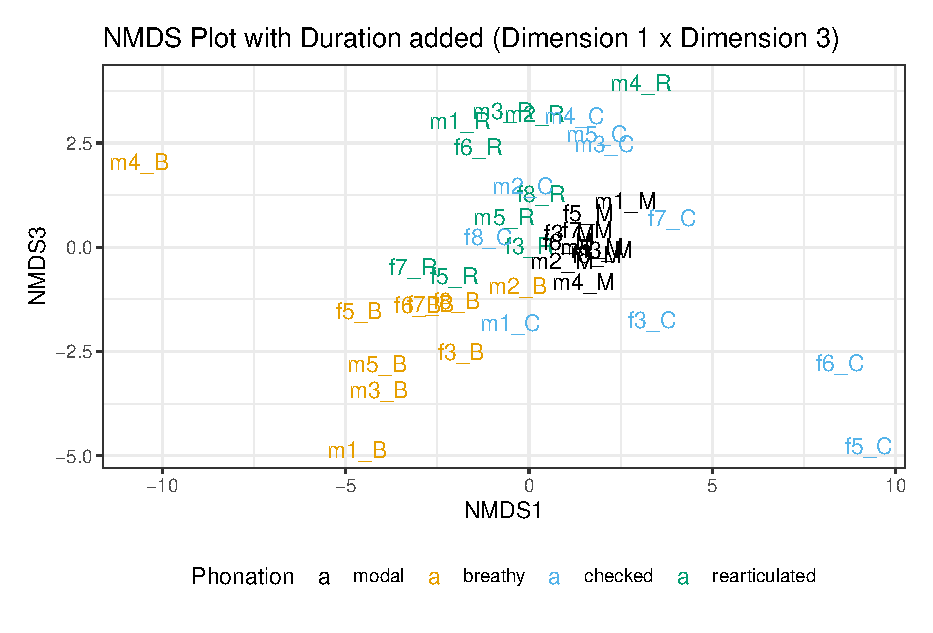
\includegraphics[width = 0.9\linewidth]{images/MDS/nmds13_dur.eps}
    \caption{Two-dimensional MDS solution showing the first and third dimensions.}
    \label{fig:nmds13}
\end{figure}

Figure~\ref{fig:nmds13} compares the first dimension to the third dimension. In this plot, We observe that breathy voice is located in the bottom left of the plot, modal voice is located in the very center of the plot, and the two types of creaky voices are located in the top right of the plot. It should be noted that the distribution of the different voice qualities follows a line from bottom-left to top-right in the plot. This suggests that the first and third dimensions capture similar information about the voice quality in SLZ.

% \begin{figure}[!h]
%     \centering
%     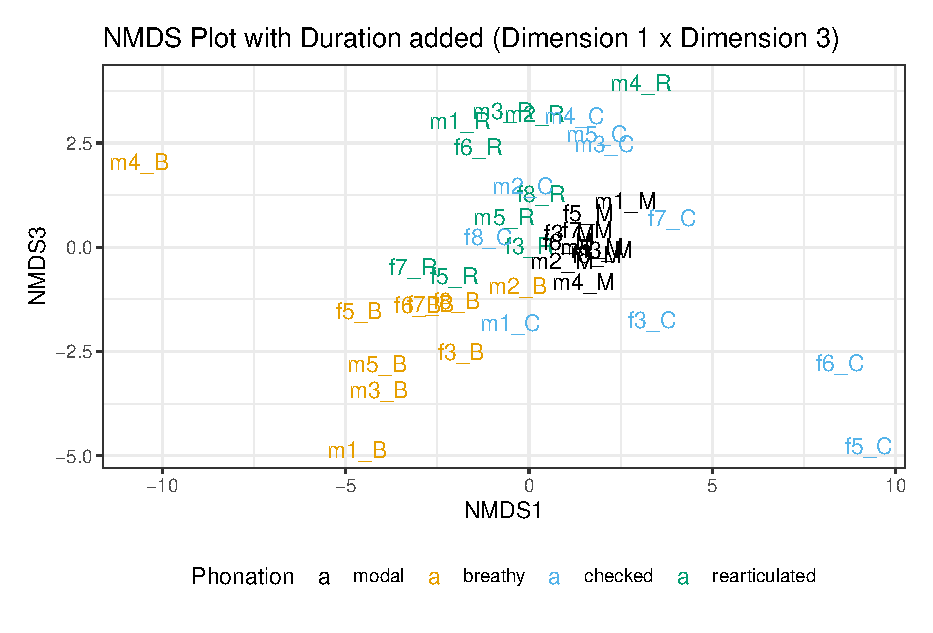
\includegraphics[width = 0.9\linewidth]{images/MDS/nmds13_dur.eps}
%     \caption{Two-dimensional MDS solution showing the first and third dimensions.}
%     \label{fig:nmds13}
% \end{figure}

Figure~\ref{fig:nmds14} shows the first dimension plotted against the fourth dimension. This plot is very similar to Figure~\ref{fig:nmds12}, with the only difference being the the fourth dimension moves the modal voice from the bottom-center of the plot to almost the exact center of the plot.

\begin{figure}[!h]
    \centering
    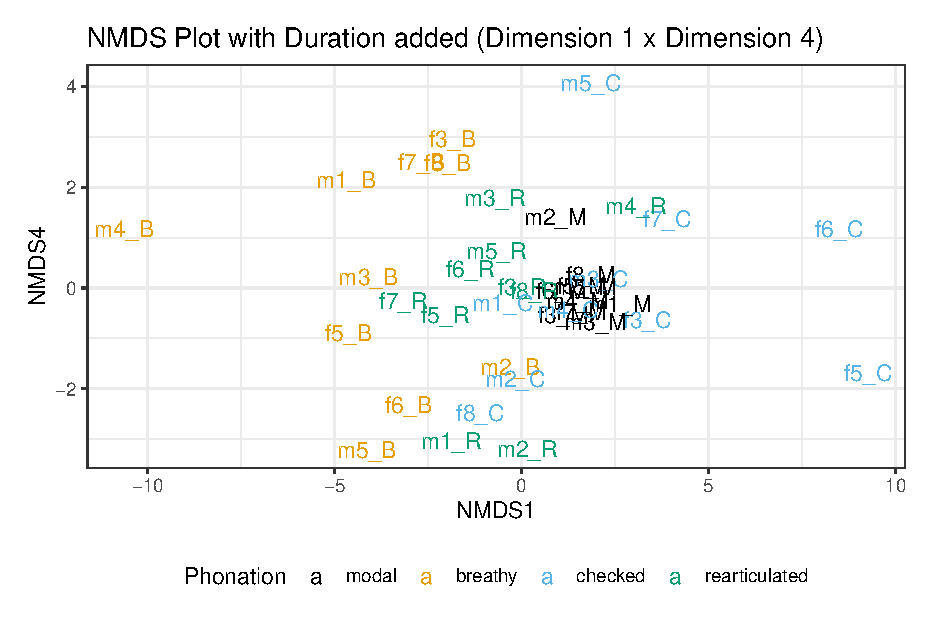
\includegraphics[width = 0.9\linewidth]{images/MDS/nmds14_dur.eps}
    \caption{Two-dimensional MDS solution showing the first and fourth dimensions.}
    \label{fig:nmds14}
\end{figure}

Figure~\ref{fig:nmds23} shows the second dimension plotted against the third dimension. This plot is essentially the same as Figure~\ref{fig:nmds13}, with that the coordinates are flipped.

\begin{figure}[!h]
    \centering
    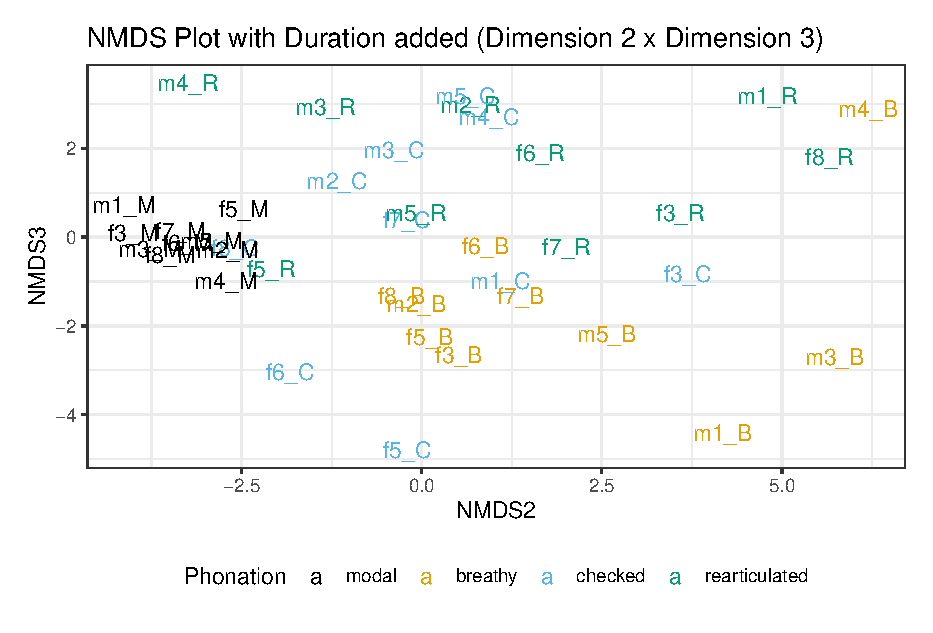
\includegraphics[width = 0.9\linewidth]{images/MDS/nmds23_dur.eps}
    \caption{Two-dimensional MDS solution showing the second and third dimensions.}
    \label{fig:nmds23}
\end{figure}

Figure~\ref{fig:nmds24} shows the second dimension plotted against the fourth dimension. This plot shows that the modal voice and nonmodal voice are separated into two different clusters, with modal voice located at the extreme left of the plot and the nonmodal voice qualities located to the right of the modal grouping. Again, as first seen in Figure~\ref{fig:nmds14}, the fourth dimension centralizes modal voice, but no discernible pattern is observed for the other phonations.

\begin{figure}[!h]
    \centering
    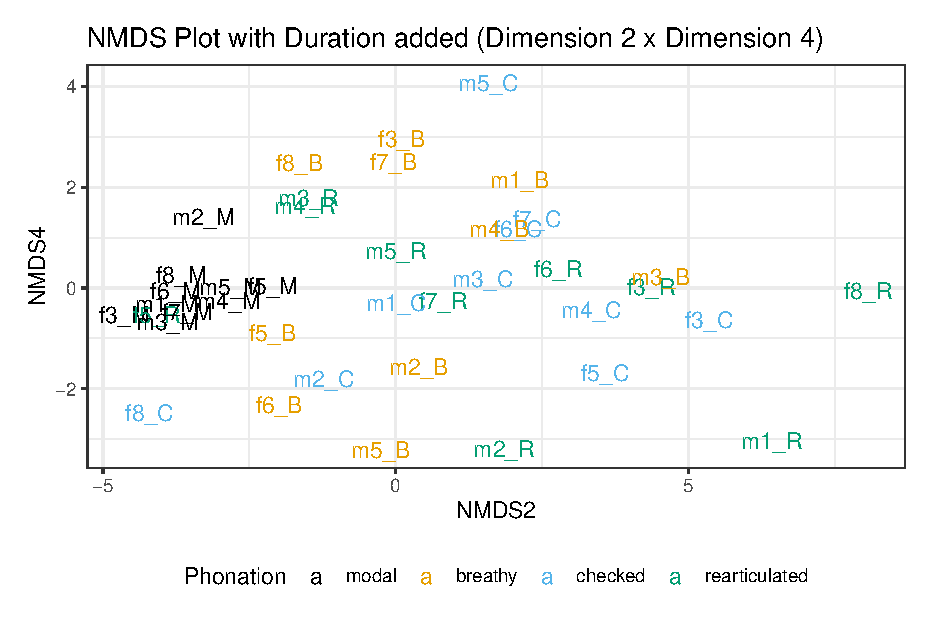
\includegraphics[width = \linewidth]{images/MDS/nmds24_dur.eps}
    \caption{Two-dimensional MDS solution showing the second and fourth dimensions.}
    \label{fig:nmds24}
\end{figure}

Figure~\ref{fig:nmds34} shows the third dimension plotted against the fourth dimension. This plot is very similar to Figure~\ref{fig:nmds14} with the exception that along the third dimension checked and rearticulated voice have swapped places. Checked voice is more centralized in the plot, while rearticulated voice is located more to the right of the plot. Again, we observe that the modal voice is located at the center of the plot.

\begin{figure}[!h]
    \centering
    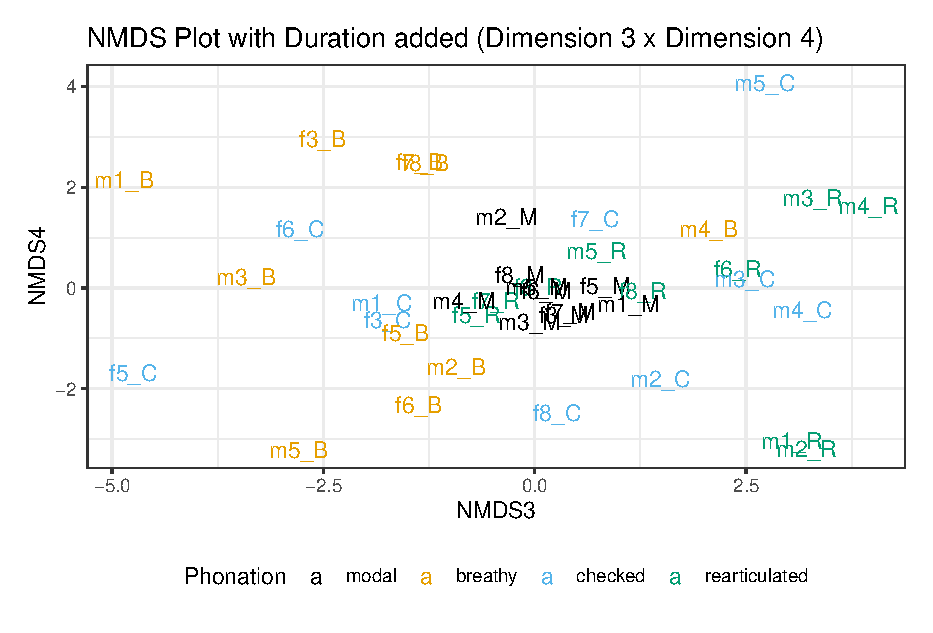
\includegraphics[width = 0.9\linewidth]{images/MDS/nmds34_dur.eps}
    \caption{Two-dimensional MDS solution showing the third and fourth dimensions.}
    \label{fig:nmds34}
\end{figure}

%--------------------------------------------------------------------------
\subsubsection{Interim summary} \label{sec:acousticlandscape:inter_sum}
%--------------------------------------------------------------------------

The plots of the MDS analysis shows us that the acoustic space of voice quality in SLZ is primarily represented by a three-dimensional space. The first dimension and third dimensions are very similar in that they capture a continuum from breathy, to modal, and finally creaky voice. This is similar to what \citet{keatingCrosslanguageAcousticSpace2023} found in their study that the first dimension captures this continuum. This continuum is very similar to the open-quotient model of voice quality put forward by \citet{gordonPhonationTypesCrosslinguistic2001}, as illustrated in Figure~\ref{fig:phonation_types}. Because of this similarly to the open-quotient model, the first and third dimensions are likely capturing the open-quotient of the glottis or something similar. 

\begin{figure}[h!]
    \centering
    \begin{tikzpicture}
        % Draw the line with arrows at both ends
        \draw[<->, line width=0.5mm] (0,0) -- (10,0);
        
        % Labels underneath the line
        \node[below] at (0,0) {[h]};
        \node[below] at (2,0) {Breathy};
        \node[below] at (5,0) {Modal};
        \node[below] at (8,0) {Creaky};
        \node[below] at (10,0) {[ʔ]};
        
        % Labels above the line
        \node[above] at (0,0) {Open Glottis};
        \node[above] at (10,0) {Closed Glottis};
    \end{tikzpicture}
    \caption{A diagram showing the relationship between breathy, modal, and creaky phonation types from \citet{gordonPhonationTypesCrosslinguistic2001}.}
    \label{fig:phonation_types}
\end{figure}

From the plots involving the second dimension, we see that this dimension separates the modals from the nonmodals. This is similar to what, we observe with the various harmonics-to-noise ratios and cepstral peak prominence (CPP) which are all measures of the the amount of noise present in the signal across various bandwidths \citep{dekromCepstrumBasedTechniqueDetermining1993,blankenshipTimingNonmodalPhonation2002,ferrerriesgoWhatMakesCepstral2020}. In addition to the amount of noise it could also be capturing the strength of the vocal fold vibration, similar to what \citet{garellekVoicingGlottalConsonants2021} found in their study of glottal consonants and non-modal phonation. In their study, they found that modal voice had the highest strength of vocal fold vibration (as measured by the Strength of Excitation) while the nonmodals had a lower strength of vocal fold vibration. This suggests that the second dimension is capturing the amount of aperiodic noise in the signal, the strength of vocal fold vibration, or both.

The fourth dimension is less clear in what it is potentially capturing. IN alll of the plots involving the fourth dimension, we see that modal voice is always located near the center of the plot, while the nonmodal voice qualities are located around this point depending on the patterns from the other dimensions. This suggests that the fourth dimension is possibly capturing something about modal voice. 

The rest of this chapter will focus on the how the different acoustic measures contribute to the different dimensions of the MDS analysis. This will be followed by a general discussion of the both the MDS analysis dimensions and the acoustic measures that are correlated with these dimesniosns. This discussion will focus on how the results of this study relate to previous work on voice quality and the implications of these results for our understanding of the acoustic space of voice quality. 

%--------------------------------------------------------------------------
\subsection{Acoustic correlates of voice quality} \label{sec:acousticlandscape:correlates}
%--------------------------------------------------------------------------

Looking at the visual representation of the dimensions is only part of the story. In order to fully understand what is going on we need to determine how the acoustic measures contribute to the An additional step to MDS analysis involves ascertaining which acoustic measures are correlated with each of the different dimensions. Table~\ref{tab:acoustic_correlates} shows these correlations. In each of the four dimensions produced by the MDS analysis, the four largest correlations for each acoustic measures are bolded. The choice to bold the four largest correlations was arbitrary and was done to make it easier to discuss each of the In the case of the first and second dimensions (D1 and D2), the acoustic measures that have weights higher than those of other parameters are in boldface (weights > 4.0). In the case of the third dimension (D3), the acoustic measures that have weights higher than those of other parameters are in boldface (weights > 3.0). 

We see that for D1, the acoustic measures that have the highest weight on the first dimension are the amplitudes for the first three formants (i.e., A1*, A2*, A3*) and HNR < 500 Hz (i.e., a harmonics-to-noise ratio for everything from 0 to 500 Hz). For D2, the acoustic measures with the highest weight are H1*$-$A1*, H1*$-$A2* (i.e., spectral-slope measures), and the amplitudes of the first two formants. For D3, we see that HNR < 1500 HZ, HNR < 2500 Hz, HNR < 3500 Hz, and Residual H1* and H2* have the highest weights.



\begin{table}[ht]
    \centering
    \caption{Correlations for each acoustic measure to the four dimensions (NMDS1, NMDS2, NMDS3, NMDS4). The four largest correlations in each dimension are bolded.} 
    \label{tab:acoustic_correlates}
    \begin{tabular}{lrrrr}
        \lsptoprule
        Acoustic Measure & NMDS1 & NMDS2 & NMDS3 & NMDS4 \\ 
        \hline
        H1*$-$H2* & -0.221 & -0.339 & 0.031 & 0.314 \\ 
        H2*$-$H4 & -0.437 & 0.239 & \textbf{-0.689} & \textbf{-0.364} \\ 
        H1*$-$A1* & \textbf{-0.828} & 0.048 & \textbf{-0.459} & 0.044 \\ 
        H1*$-$A2* & \textbf{-0.855} & -0.067 & -0.343 & 0.114 \\ 
        H1*$-$A3* & \textbf{-0.809} & -0.218 & -0.297 & 0.126 \\ 
        H4*$-$H2k* & -0.452 & -0.598 & 0.294 & \textbf{0.366} \\ 
        H2k*$-$H5k* & 0.152 & 0.023 & 0.101 & 0.057 \\ 
        residual H1* & -0.290 & -0.443 & \textbf{-0.722} & 0.084 \\ 
        H2* & -0.157 & -0.555 & \textbf{-0.679} & 0.114 \\ 
        H4* & 0.295 & \textbf{-0.778} & 0.078 & \textbf{0.479} \\ 
        A1* & 0.756 & -0.549 & 0.092 & 0.124 \\ 
        A2* & \textbf{0.779} & -0.476 & -0.103 & 0.086 \\ 
        A3* & 0.735 & -0.416 & -0.211 & 0.093 \\ 
        CPP & -0.590 & -0.606 & 0.209 & -0.179 \\ 
        HNR < 500 Hz & -0.513 & \textbf{-0.792} & 0.152 & -0.202 \\ 
        HNR < 1500 Hz & -0.275 & \textbf{-0.799} & 0.323 & -0.290 \\ 
        HNR < 2500 Hz & -0.327 & -0.714 & 0.391 & -0.348 \\ 
        HNR < 3500 Hz & -0.446 & -0.644 & 0.393 & -0.356 \\ 
        SoE & -0.013 & -0.741 & -0.238 & 0.145 \\ 
        SHR & 0.144 & -0.176 & 0.122 & \textbf{-0.597} \\ 
        Energy & -0.080 & \textbf{-0.793} & -0.015 & 0.341 \\ 
        Duration & -0.622 & 0.539 & 0.257 & 0.030 \\ 
        \lspbottomrule
    \end{tabular}
    % \begin{tabular}{lrrr}
    % \hline
    % Acoustic Measure & D1 & D2 & D3 \\ 
    % \hline
    % H1*$-$H2* & 1.03 & 1.01 & 0.39 \\ 
    % H2*$-$H4 & 1.15 & 3.98 & 2.13 \\ 
    % H1*$-$A1* & 2.22 & \textbf{5.15} & 1.84 \\ 
    % H1*$-$A2* & 2.93 & \textbf{4.66} & 1.00 \\ 
    % H1*$-$A3* & 2.37 & 3.24 & 0.90 \\ 
    % H4*$-$H2k* & 1.47 & 0.31 & 1.59 \\ 
    % H2k*$-$H5k* & 3.73 & 0.73 & 0.84 \\ 
    % residual H1* & 1.75 & 0.97 & \textbf{4.24} \\ 
    % H2* & 1.76 & 0.94 & \textbf{4.09} \\ 
    % H4* & 0.79 & \textbf{4.28} & 0.10 \\ 
    % A1* & \textbf{4.96} & \textbf{5.48} & 0.17 \\ 
    % A2* & \textbf{5.30} & \textbf{4.90} & 1.38 \\ 
    % A3* & \textbf{4.54} & 2.91 & 1.11 \\ 
    % CPP & \textbf{4.08} & 0.10 & 1.68 \\ 
    % HNR < 500 Hz & \textbf{5.66} & 1.47 & 1.81 \\ 
    % HNR < 1500 Hz & 3.95 & 2.68 & \textbf{3.08} \\ 
    % HNR < 2500 Hz & 3.15 & 1.63 & \textbf{3.42} \\ 
    % HNR < 3500 Hz & 2.86 & 0.55 & \textbf{3.19} \\ 
    % Strength of Excitation & 2.09 & 0.78 & 0.36 \\ 
    % SHR & 2.39 & 0.50 & 0.47 \\ 
    % Energy & 2.22 & 3.91 & 0.64 \\ 
    % \hline
    % \end{tabular}
\end{table}

%--------------------------------------------------------------------------
\section{Discussion} \label{sec:acousticlandscape:discussion}
%--------------------------------------------------------------------------

The results of the MDS analysis show that the acoustic space in which SLZ's voice quality occupies is similar to other languages. Similar to what \citet{keatingCrosslanguageAcousticSpace2023} found in their study, the first dimension appears to roughly be similar to the open quotient of the glottis as proposed by \citet{gordonPhonationTypesCrosslinguistic2001}. In this model, voice quality is seen as the result of the glottis being more open or closed during phonation. The more open the glottis, the more breathy the phonation will be. The more closed the glottis, the more creaky the phonation will be. This model from \citet{gordonPhonationTypesCrosslinguistic2001} is shown in Figure~\ref{fig:phonation_types}.

\begin{figure}[h!]
    \centering
    \begin{tikzpicture}
        % Draw the line with arrows at both ends
        \draw[<->, line width=0.5mm] (0,0) -- (10,0);
        
        % Labels underneath the line
        \node[below] at (0,0) {[h]};
        \node[below] at (2,0) {Breathy};
        \node[below] at (5,0) {Modal};
        \node[below] at (8,0) {Creaky};
        \node[below] at (10,0) {[ʔ]};
        
        % Labels above the line
        \node[above] at (0,0) {Open Glottis};
        \node[above] at (10,0) {Closed Glottis};
    \end{tikzpicture}
    \caption{A diagram showing the relationship between breathy, modal, and creaky phonation types. Based on \citet{gordonPhonationTypesCrosslinguistic2001}.}
    \label{fig:phonation_types}
\end{figure}

As mentioned above, the measures that contribute the most to this first dimension are the amplitudes of the first three formants, CPP, and Harmonics-to-Noise Ratio < 500 Hz. Interestingly, even though this dimension is similar to the open-quotient model put forward by \citet{gordonPhonationTypesCrosslinguistic2001}, we do not observe measures traditionally associated with the open-quotient (i.e., spectral-slope). Instead of seeing traditional spectral-slope measures, we find the three formant amplitudes used to normalize the amplitude of the fundamental like in the measures H1*$-$A1*, H1*$-$A2*, and H1*$-$A3*. This suggests that the first dimension is more about the formants' amplitude than the signal's spectral-slope. This is combined with CPP and HNR < 500 Hz, which measures the harmonics-to-noise ratio for the first 500 Hz of the signal. This suggests that the first dimension is also concerned with the amount of noise in the signal.

The second dimension divides the space into modal versus nonmodal voice quality. The acoustic measures that contribute the most weight to this dimension are the spectral-slope measures H1*$-$A1* and H1*$-$A2* and the harmonic amplitudes of H4*, A1*, and A2*. This suggests that the second dimension is more about the spectral-slope of the signal than about the amount of noise in the signal. This is interesting given that traditional spectral-slope measures are associated with the open-quotient model of voice quality \citep{holmbergComparisonsAerodynamicElectroglottographic1995,kreimanMeasuresGlottalSource2007,garellekModelingVoiceSource2016,garellekPhoneticsVoice2019,chaiH1H2Acoustic2022}.

The third dimension adds more information on nonmodal voice quality. Figure~\ref{fig:nmds13} and Figure~\ref{fig:nmds23}, this third dimension separates the breathy voice from the other nonmodal phonation types. The measures contributing the most to this dimension are the harmonics-to-noise ratio for the first 1500 Hz, 2500 Hz, and 3500 Hz. In addition, the residual H1* and H2* have the highest weights, which is interesting given that residual H1* has been argued to be a more robust measure of the spectral-slope of the signal than traditional spectral-slope measures \citep{chaiH1H2Acoustic2022,brinkerhoffResidualH1Measure2024}. Furthermore, as discussed in Chapter~\ref{ch:residual_h1}, residual H1* represents the voice quality in SLZ better than H1*$-$H2* and H1*$-$A3*. This dimension is characterized by the harmonics-to-noise ratios for the first 1500 Hz, 2500 Hz, and 3500 Hz. This suggests that the third dimension is more about the signal's spectral quality than about the formants' amplitude. This is combined with residual H1* and H2*, which are measures of the spectral-slope of the signal.

%--------------------------------------------------------------------------
\section{Conclusion} \label{sec:acousticlandscape:conclusion}
%--------------------------------------------------------------------------

Although the discussion has predominately been about the weights of the measures that contribute to the different dimensions, it is important to note that the measures are not independent of each other. Instead, all of the measures contribute to the acoustic space of voice quality in SLZ to some extent or another. Just because a measure has a low weight does not mean that it does not contribute to the acoustic space, but it is still important to understand the acoustic space in SLZ. Rather than thinking of the measures as independent of each other, it is better to think of them as a group of measures that work together to create the acoustic space of voice quality in SLZ. This is especially true given the fact that the MDS analysis is a reduction of the data to a few dimensions. This analysis offers a snapshot of the voice quality acoustic space in SLZ, but is not the full picture. 

Additionally, as will be discussed in Chapter~\ref{ch:bagging}, another way in which we can determine which measures are the most important is by performing a bootstrap aggregating version of a classification and regression tree analysis \citep{breimanClassificationRegressionTrees1986,breimanBaggingPredictors1996}.